\newcommand{\titulus}{\nomenFesti{S. Callisti I, Papæ \& Martyris.}
\dies{Die 14. Octobris.}}
\newcommand{\sineobmv}{Sine officium B.M.V.}
\newcommand{\oratio}{\pars{Oratio.}

\noindent Preces pópuli tui, quǽsumus, Dómine, cleménter exáudi, ut beáti Callísti, papæ, méritis adiuvémur, cuius passióne lætámur.

\pars{Pro pace in universo mundo.} \scriptura{Sir. 50, 25; 2 Esdr. 4, 20; \textbf{H416}}

\vspace{-4mm}

\antiphona{II D}{temporalia/ant-dapacemdomine.gtex}

\vfill

\noindent Deus, a quo sancta desidéria, recta consília et iusta sunt ópera: da servis tuis illam, quam mundus dare non potest, pacem; ut et corda nostra mandátis tuis dédita, et hóstium subláta formídine, témpora sint tua protectióne tranquílla.

\noindent Per Dóminum nostrum Iesum Christum, Fílium tuum, qui tecum vivit et regnat in unitáte Spíritus Sancti, Deus, per ómnia sǽcula sæculórum.

\noindent \Rbardot{} Amen.}
\newcommand{\invitatorium}{\pars{Invitatorium.}

\vspace{-4mm}

\antiphona{E}{temporalia/inv-regemmartyrumsimplex.gtex}}
\newcommand{\hymnusmatutinum}{\pars{Hymnus}

\cuminitiali{I}{temporalia/hym-BeateMartyr.gtex}}
\newcommand{\matversus}{\noindent \Vbardot{} Fili mi, atténde ad sapiéntiam meam.

\noindent \Rbardot{} Et prudéntiæ meæ inclína aurem tuam.}
\newcommand{\lectioi}{\pars{Lectio I.} \scriptura{Zach. 1, 1-16}

\noindent Incipit liber Zacharíæ prophétæ.

\noindent In mense octávo, in anno secúndo Daríi, factum est verbum Dómini ad Zacharíam fílium Barachíæ fílii Addo prophétam dicens: «Irátus est Dóminus super patres vestros iracúndia. Et dices ad eos: Hæc dicit Dóminus exercítuum: Convertímini ad me, ait Dóminus exercítuum; et convértar ad vos, dicit Dóminus exercítuum. Ne sitis sicut patres vestri, ad quos clamábant prophétæ prióres dicéntes: Hæc dicit Dóminus exercítuum: Convertímini de viis vestris malis et de cogitatiónibus vestris malis; et non audiérunt, neque attendérunt ad me, dicit Dóminus. Patres vestri ubi sunt? Et prophétæ numquid in sempitérnum vivent? Verúmtamen verba mea et præcépta mea, quæ mandávi servis meis prophétis, numquid non attigérunt patres vestros? Et convérsi sunt et dixérunt: “Sicut cogitávit Dóminus exercítuum fácere nobis, secúndum vias nostras et secúndum adinventiónes nostras fecit nobis”».

\noindent {\color{gray} In die vicésima et quarta undécimi mensis, qui est mensis Sabath, in anno secúndo Daríi, factum est verbum Dómini ad Zacharíam fílium Barachíæ fílii Addo prophétam dicens: «Vidi per noctem, et ecce vir sedens super equum rufum et ipse stabat inter myrtéta, quæ erant in profúndo; et post eum equi rufi, fulvi et albi. Et dixi: “Quid sunt isti, dómine mi?”. Et dixit ad me ángelus, qui loquebátur in me: “Ego osténdam tibi quid sint isti”. Et respóndit vir, qui stabat inter myrtéta, et dixit: “Isti sunt quos misit Dóminus, ut perambulárent terram”. Et respondérunt ángelo Dómini, qui stabat inter myrtéta, et dixérunt: “Perambulávimus terram, et ecce omnis terra habitátur et quiéscit”.}

\noindent Et respóndit ángelus Dómini et dixit: “Dómine exercítuum, úsquequo tu non miseréberis Ierúsalem et úrbium Iudæ, quibus irátus es? Iste septuagésimus annus est!”. Et respóndit Dóminus ángelo, qui loquebátur in me verba bona, verba consolatória. Et dixit ad me ángelus, qui loquebátur in me: “Clama dicens: Hæc dixit Dóminus exercítuum: Zelátus sum Ierúsalem et Sion zelo magno, sed ira magna ego iráscor super gentes opuléntas, quia ego irátus sum parum, ipsi vero adiuvérunt in malum. Proptérea hæc dicit Dóminus: Revértar ad Ierúsalem in misericórdiis. Domus mea ædificábitur in ea, ait Dóminus exercítuum, et perpendículum extendétur super Ierúsalem.}
\newcommand{\responsoriumi}{\pars{Responsorium 1.} \scriptura{\Rbardot{} Ier. 31, 11.12 \Vbardot{} Ps. 4, 8; \textbf{H418}}

\vspace{-5mm}

\responsorium{III}{temporalia/resp-redemitdominus-CROCHU.gtex}{}}
\newcommand{\lectioii}{\pars{Lectio II.} \scriptura{Cap. 13: CSEL 3, 346-347}

\noindent Ex Tractátu sancti Cypriáni epíscopi et mártyris ad Fortunátum.

\noindent \emph{Non sunt condígnæ passiónes huius témporis ad superventúram claritúdinem quæ revelábitur in nobis.} Quis ergo non ómnibus modis elabóret ad claritátem tantam perveníre, ut amícus Dei fiat, ut cum Christo statim gáudeat, ut post torménta et supplícia terréna prǽmia divína percípiat? Si milítibus sæculáribus gloriósum est ut hoste devícto rédeant in pátriam triumphántes, quanto pótior et maior est glória victo diábolo ad paradísum triumphántem redíre et, unde Adam peccátor eiéctus est, illuc prostráto eo qui ante decéperat tropǽa victrícia reportáre, offérre Dómino acceptíssimum munus incorrúptam fidem, virtútem mentis incólumem, laudem devotiónis illústrem, comitári eum cum veníre cœ́perit vindíctam de inimícis receptúrus, láteri eius assístere cum séderit iudicatúrus, coherédem Christi fíeri, ángelis coæquári, cum patriárchis, cum apóstolis, cum prophétis cæléstis regni possessióne lætári.}
\newcommand{\responsoriumii}{\pars{Responsorium 2.} \scriptura{\textbf{H373}}

\vspace{-5mm}

\responsorium{III}{temporalia/resp-istecognovit-CROCHU.gtex}{}

\vfill
\pagebreak

\rubrica{vel ad libitum:}

\vspace{3mm}

\pars{Responsorium 2.}

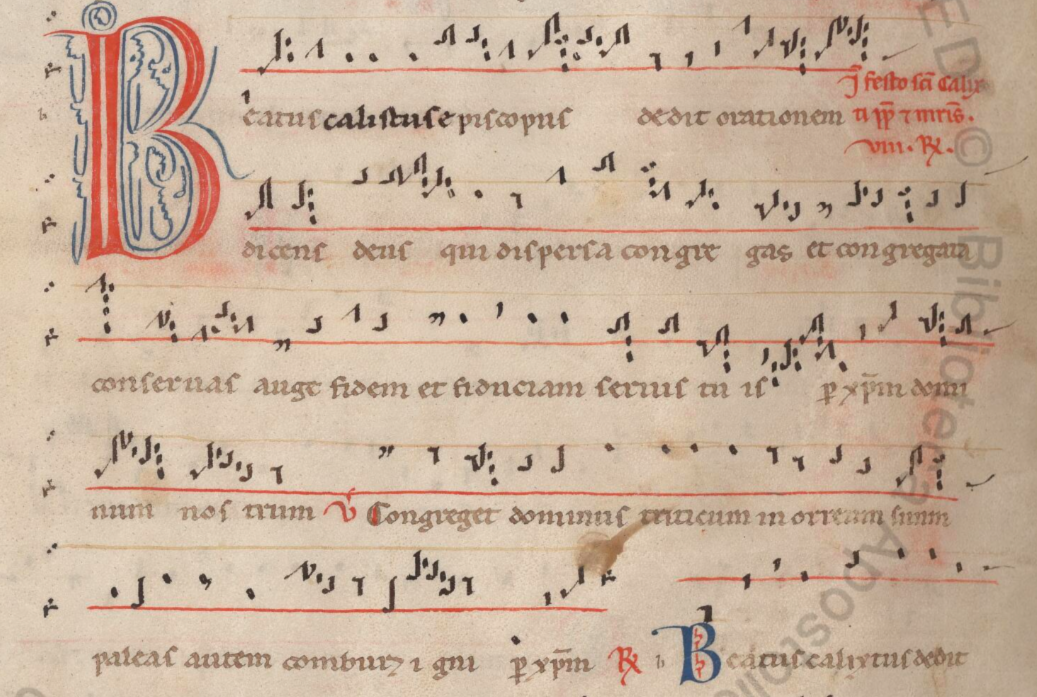
\includegraphics[width=17cm]{pic-beatuscallistus.png}}
\newcommand{\lectioiii}{\pars{Lectio III.}

\noindent Has cogitatiónes quæ persecútio potest víncere, quæ possunt torménta superáre? Durat fortis et stábilis religiósis meditatiónibus fundáta mens et advérsus omnes diáboli terróres et minas mundi ánimus immóbilis perstat, quem futurórum fides certa et sólida corróborat. Claudúntur in persecutiónibus terræ, sed patet cælum; minátur antichrístus, sed Christus tuétur; mors infértur, sed immortálitas séquitur. Quanta est dígnitas et quanta secúritas exíre hinc lætum, exíre inter pressúras et angústias gloriósum, cláudere in moménto óculos, quibus hómines videbántur et mundus, aperíre eósdem statim, ut Deus videátur et Christus. Tam felíciter migrándi quanta velócitas. Terris repénte subtráheris, ut in regnis cæléstibus reponáris.

\noindent Hæc opórtet mente et cogitatióne complécti, hæc die ac nocte meditári. Si talem persecútio invénerit Dei mílitem, vinci non póterit virtus ad prœ́lium prompta. Vel si arcessítio ante prævénerit, sine prǽmio non erit fides quæ erat ad martýrium præparáta; sine damno témporis merces Deo iúdice rédditur; in persecutióne milítia, in pace consciéntia coronátur.}
\newcommand{\responsoriumiii}{\pars{Responsorium 3.} \scriptura{\Rbardot{} Ps. 8, 6-8 \Vbardot{} Ps. 20, 4; \textbf{H374}}

\vspace{-5mm}

\responsorium{VII}{temporalia/resp-gloriaethonore-CROCHU-cumdox.gtex}{}}
\newcommand{\hymnuslaudes}{\pars{Hymnus}

\cuminitiali{VI}{temporalia/hym-MartyrDei.gtex}}
\newcommand{\lectiobrevis}{\pars{Lectio Brevis.} \scriptura{2 Cor. 1, 3-5}

\noindent Benedíctus Deus et Pater Dómini nostri Iesu Christi, Pater misericordiárum et Deus totíus consolatiónis, qui consolátur nos in omni tribulatióne nostra, ut possímus et ipsi consolári eos, qui in omni pressúra sunt, per exhortatiónem, qua exhortámur et ipsi a Deo; quóniam, sicut abúndant passiónes Christi in nobis, ita per Christum abúndat et consolátio.}
\newcommand{\responsoriumbreve}{\pars{Responsorium breve.} \scriptura{Ex. 15, 2}

\cuminitiali{VI}{temporalia/resp-fortitudomeaetlausmea.gtex}}
\newcommand{\preces}{\noindent Fratres, Salvatórem nostrum, testem fidélem, per mártyres interféctos propter verbum Dei,~\gredagger{} celebrémus, clamántes:

\Rbardot{} Redemísti nos Deo in sánguine tuo.

\noindent Per mártyres tuos, qui líbere mortem in testimónium fídei sunt ampléxi,~\gredagger{} da nobis, Dómine, veram spíritus libertátem.

\Rbardot{} Redemísti nos Deo in sánguine tuo.

\noindent Per mártyres tuos, qui fidem usque ad sánguinem sunt conféssi,~\gredagger{} da nobis, Dómine, puritátem fideíque constántiam.

\Rbardot{} Redemísti nos Deo in sánguine tuo.

\noindent Per mártyres tuos, qui, sustinéntes crucem, tua vestígia sunt secúti,~\gredagger{} da nobis, Dómine, ærúmnas vitæ fórtiter sustinére.

\Rbardot{} Redemísti nos Deo in sánguine tuo.

\noindent Per mártyres tuos, qui stolas suas lavérunt in sánguine Agni,~\gredagger{} da nobis, Dómine, omnes insídias carnis mundíque devíncere.

\Rbardot{} Redemísti nos Deo in sánguine tuo.}
\newcommand{\benedictus}{\pars{Canticum Zachariæ.} \scriptura{Io. 12, 35; \textbf{H375}}

\vspace{-4mm}

\antiphona{III a}{temporalia/ant-quisequiturmenonambulat.gtex}

%\vspace{-2mm}

\scriptura{Lc. 1, 68-79}

\vspace{-2mm}

\cantusSineNeumas
\initiumpsalmi{temporalia/benedictus-initium-iii-a-auto.gtex}

%\vspace{-1.5mm}

\input{temporalia/benedictus-iii-a.tex} \Abardot{}}
\newcommand{\benedicamuslaudes}{\cuminitiali{}{temporalia/benedicamus-memoria-laudes.gtex}}
\newcommand{\hebdomada}{infra Hebdom. XXVIII per Annum.}
%\newcommand{\hiemalis}{Hiemalis}
\newcommand{\matud}{Matutinum Hebdomadae D}
\newcommand{\matubd}{Matutinum Hebdomadae B vel D}
\newcommand{\laudd}{Laudes Hebdomadae D}
\newcommand{\laudbd}{Laudes Hebdomadae B vel D}

% LuaLaTeX

\documentclass[a4paper, twoside, 12pt]{article}
\usepackage[latin]{babel}
%\usepackage[landscape, left=3cm, right=1.5cm, top=2cm, bottom=1cm]{geometry} % okraje stranky
%\usepackage[landscape, a4paper, mag=1166, truedimen, left=2cm, right=1.5cm, top=1.6cm, bottom=0.95cm]{geometry} % okraje stranky
\usepackage[landscape, a4paper, mag=1400, truedimen, left=0.5cm, right=0.5cm, top=0.5cm, bottom=0.5cm]{geometry} % okraje stranky

\usepackage{fontspec}
\setmainfont[FeatureFile={junicode.fea}, Ligatures={Common, TeX}, RawFeature=+fixi]{Junicode}
%\setmainfont{Junicode}

% shortcut for Junicode without ligatures (for the Czech texts)
\newfontfamily\nlfont[FeatureFile={junicode.fea}, Ligatures={Common, TeX}, RawFeature=+fixi]{Junicode}

\usepackage{multicol}
\usepackage{color}
\usepackage{lettrine}
\usepackage{fancyhdr}

% usual packages loading:
\usepackage{luatextra}
\usepackage{graphicx} % support the \includegraphics command and options
\usepackage{gregoriotex} % for gregorio score inclusion
\usepackage{gregoriosyms}
\usepackage{wrapfig} % figures wrapped by the text
\usepackage{parcolumns}
\usepackage[contents={},opacity=1,scale=1,color=black]{background}
\usepackage{tikzpagenodes}
\usepackage{calc}
\usepackage{longtable}
\usetikzlibrary{calc}

\setlength{\headheight}{14.5pt}

% Commands used to produce a typical "Conventus" booklet

\newenvironment{titulusOfficii}{\begin{center}}{\end{center}}
\newcommand{\dies}[1]{#1

}
\newcommand{\nomenFesti}[1]{\textbf{\Large #1}

}
\newcommand{\celebratio}[1]{#1

}

\newcommand{\hora}[1]{%
\vspace{0.5cm}{\large \textbf{#1}}

\fancyhead[LE]{\thepage\ / #1}
\fancyhead[RO]{#1 / \thepage}
\addcontentsline{toc}{subsection}{#1}
}

% larger unit than a hora
\newcommand{\divisio}[1]{%
\begin{center}
{\Large \textsc{#1}}
\end{center}
\fancyhead[CO,CE]{#1}
\addcontentsline{toc}{section}{#1}
}

% a part of a hora, larger than pars
\newcommand{\subhora}[1]{
\begin{center}
{\large \textit{#1}}
\end{center}
%\fancyhead[CO,CE]{#1}
\addcontentsline{toc}{subsubsection}{#1}
}

% rubricated inline text
\newcommand{\rubricatum}[1]{\textit{#1}}

% standalone rubric
\newcommand{\rubrica}[1]{\vspace{3mm}\rubricatum{#1}}

\newcommand{\notitia}[1]{\textcolor{red}{#1}}

\newcommand{\scriptura}[1]{\hfill \small\textit{#1}}

\newcommand{\translatioCantus}[1]{\vspace{1mm}%
{\noindent\footnotesize \nlfont{#1}}}

% pruznejsi varianta nasledujiciho - umoznuje nastavit sirku sloupce
% s prekladem
\newcommand{\psalmusEtTranslatioB}[3]{
  \vspace{0.5cm}
  \begin{parcolumns}[colwidths={2=#3}, nofirstindent=true]{2}
    \colchunk{
      \input{#1}
    }

    \colchunk{
      \vspace{-0.5cm}
      {\footnotesize \nlfont
        \input{#2}
      }
    }
  \end{parcolumns}
}

\newcommand{\psalmusEtTranslatio}[2]{
  \psalmusEtTranslatioB{#1}{#2}{8.5cm}
}


\newcommand{\canticumMagnificatEtTranslatio}[1]{
  \psalmusEtTranslatioB{#1}{temporalia/extra-adventum-vespers/magnificat-boh.tex}{12cm}
}
\newcommand{\canticumBenedictusEtTranslatio}[1]{
  \psalmusEtTranslatioB{#1}{temporalia/extra-adventum-laudes/benedictus-boh.tex}{10.5cm}
}

% volne misto nad antifonami, kam si zpevaci dokresli neumy
\newcommand{\hicSuntNeumae}{\vspace{0.5cm}}

% prepinani mista mezi notovymi osnovami: pro neumovane a neneumovane zpevy
\newcommand{\cantusCumNeumis}{
  \setgrefactor{17}
  \global\advance\grespaceabovelines by 5mm%
}
\newcommand{\cantusSineNeumas}{
  \setgrefactor{17}
  \global\advance\grespaceabovelines by -5mm%
}

% znaky k umisteni nad inicialu zpevu
\newcommand{\superInitialam}[1]{\gresetfirstlineaboveinitial{\small {\textbf{#1}}}{\small {\textbf{#1}}}}

% pars officii, i.e. "oratio", ...
\newcommand{\pars}[1]{\textbf{#1}}

\newenvironment{psalmus}{
  \setlength{\parindent}{0pt}
  \setlength{\parskip}{5pt}
}{
  \setlength{\parindent}{10pt}
  \setlength{\parskip}{10pt}
}

%%%% Prejmenovat na latinske:
\newcommand{\nadpisZalmu}[1]{
  \hspace{2cm}\textbf{#1}\vspace{2mm}%
  \nopagebreak%

}

% mode, score, translation
\newcommand{\antiphona}[3]{%
\hicSuntNeumae
\superInitialam{#1}
\includescore{#2}

#3
}
 % Often used macros

\newcommand{\annusEditionis}{2021}

%%%% Vicekrat opakovane kousky

\newcommand{\anteOrationem}{
  \rubrica{Ante Orationem, cantatur a Superiore:}

  \pars{Supplicatio Litaniæ.}

  \cuminitiali{}{temporalia/supplicatiolitaniae.gtex}

  \pars{Oratio Dominica.}

  \cuminitiali{}{temporalia/oratiodominica.gtex}

  \rubrica{Deinde dicitur ab Hebdomadario:}

  \cuminitiali{}{temporalia/dominusvobiscum-solemnis.gtex}

  \rubrica{In choro monialium loco Dominus vobiscum dicitur:}

  \sineinitiali{temporalia/domineexaudi.gtex}
}

\setlength{\columnsep}{30pt} % prostor mezi sloupci

%%%%%%%%%%%%%%%%%%%%%%%%%%%%%%%%%%%%%%%%%%%%%%%%%%%%%%%%%%%%%%%%%%%%%%%%%%%%%%%%%%%%%%%%%%%%%%%%%%%%%%%%%%%%%
\begin{document}

% Here we set the space around the initial.
% Please report to http://home.gna.org/gregorio/gregoriotex/details for more details and options
\grechangedim{afterinitialshift}{2.2mm}{scalable}
\grechangedim{beforeinitialshift}{2.2mm}{scalable}
\grechangedim{interwordspacetext}{0.22 cm plus 0.15 cm minus 0.05 cm}{scalable}%
\grechangedim{annotationraise}{-0.2cm}{scalable}

% Here we set the initial font. Change 38 if you want a bigger initial.
% Emit the initials in red.
\grechangestyle{initial}{\color{red}\fontsize{38}{38}\selectfont}

\pagestyle{empty}

%%%% Titulni stranka
\begin{titulusOfficii}
\ifx\titulus\undefined
\nomenFesti{Feria III \hebdomada{}}
\else
\titulus
\fi
\end{titulusOfficii}

\vfill

\begin{center}
%Ad usum et secundum consuetudines chori \guillemotright{}Conventus Choralis\guillemotleft.

%Editio Sancti Wolfgangi \annusEditionis
\end{center}

\scriptura{}

\pars{}

\pagebreak

\renewcommand{\headrulewidth}{0pt} % no horiz. rule at the header
\fancyhf{}
\pagestyle{fancy}

\cantusSineNeumas

\hora{Ad Matutinum.} %%%%%%%%%%%%%%%%%%%%%%%%%%%%%%%%%%%%%%%%%%%%%%%%%%%%%

\vspace{2mm}

\cuminitiali{}{temporalia/dominelabiamea.gtex}

\vfill
%\pagebreak

\vspace{2mm}

\ifx\invitatorium\undefined
\pars{Invitatorium.} \scriptura{Lc. 24, 34; Psalmus 94; \textbf{H232}}

\vspace{-6mm}

\antiphona{VI}{temporalia/inv-surrexitdominusvere.gtex}
\else
\invitatorium
\fi

\vfill
\pagebreak

\ifx\hymnusmatutinum\undefined
\pars{Hymnus}

\cuminitiali{VIII}{temporalia/hym-LaetareCaelum.gtex}
\else
\hymnusmatutinum
\fi

\vspace{-3mm}

\vfill
\pagebreak

\ifx\matutinum\undefined
\ifx\matua\undefined
\else
% MAT A
\pars{Psalmus 1.}

\vspace{-4mm}

\antiphona{II D}{temporalia/ant-alleluia-turco7.gtex}

%\vspace{-2mm}

\scriptura{Ps. 9, 22-32}

%\vspace{-2mm}

\initiumpsalmi{temporalia/ps9xxii_xxxii-initium-ii-D-auto.gtex}

\input{temporalia/ps9xxii_xxxii-ii-D.tex}

\vfill
\pagebreak

\pars{Psalmus 2.} \scriptura{Ps. 9, 33-39}

%\vspace{-2mm}

\initiumpsalmi{temporalia/ps9xxxiii_xxxix-initium-ii-D-auto.gtex}

\input{temporalia/ps9xxxiii_xxxix-ii-D.tex}

\vfill
\pagebreak

\pars{Psalmus 3.} \scriptura{Ps. 11}

%\vspace{-2mm}

\initiumpsalmi{temporalia/ps11-initium-ii-D-auto.gtex}

\input{temporalia/ps11-ii-D.tex}

\vfill

\antiphona{}{temporalia/ant-alleluia-turco7.gtex}

\vfill
\pagebreak
\fi
\ifx\matub\undefined
\else
% MAT B
\pars{Psalmus 1.}

\vspace{-4mm}

\antiphona{VI F}{temporalia/ant-alleluia-turco6.gtex}

%\vspace{-2mm}

\scriptura{Ps. 36, 1-11}

%\vspace{-2mm}

\initiumpsalmi{temporalia/ps36i_xi-initium-vi-F-auto.gtex}

\input{temporalia/ps36i_xi-vi-F.tex}

\vfill
\pagebreak

\pars{Psalmus 2.}

\scriptura{Ps. 36, 12-29}

\vspace{-2mm}

\initiumpsalmi{temporalia/ps36xii_xxix-initium-vi-F-auto.gtex}

\input{temporalia/ps36xii_xxix-vi-F.tex}

\vfill
\pagebreak

\pars{Psalmus 3.}

\scriptura{Ps. 36, 30-40}

%\vspace{-2mm}

\initiumpsalmi{temporalia/ps36iii-initium-vi-F-auto.gtex}

\input{temporalia/ps36iii-vi-F.tex}

\antiphona{}{temporalia/ant-alleluia-turco6.gtex}

\vfill
\pagebreak
\fi
\ifx\matuc\undefined
\else
% MAT C
\pars{Psalmus 1.}

\vspace{-4mm}

\antiphona{I g\textsuperscript{5}}{temporalia/ant-alleluia-auglx2.gtex}

%\vspace{-2mm}

\scriptura{Ps. 67, 2-11}

\initiumpsalmi{temporalia/ps67i-initium-i-g5.gtex}

\input{temporalia/ps67i-i-g.tex}

\vfill
\pagebreak

\pars{Psalmus 2.}

\scriptura{Ps. 67, 12-24}

%\vspace{-2mm}

\initiumpsalmi{temporalia/ps67ii-initium-i-g5.gtex}

\input{temporalia/ps67ii-i-g.tex}

\vfill
\pagebreak

\pars{Psalmus 3.}

\scriptura{Ps. 67, 25-36}

\initiumpsalmi{temporalia/ps67iii-initium-i-g5.gtex}

\input{temporalia/ps67iii-i-g.tex}

\vfill

\antiphona{}{temporalia/ant-alleluia-auglx2.gtex}

\vfill
\pagebreak
\fi
\ifx\matud\undefined
\else
% MAT D
\pars{Psalmus 1.}

\vspace{-4mm}

\antiphona{I d\textsuperscript{3}}{temporalia/ant-alleluia-auglx6.gtex}

%\vspace{-2mm}

\scriptura{Ps. 101, 2-12}

%\vspace{-2mm}

\initiumpsalmi{temporalia/ps101ii_xii-initium-i-d3-auto.gtex}

\input{temporalia/ps101ii_xii-i-d3.tex}

\vfill
\pagebreak

\pars{Psalmus 2.} \scriptura{Ps. 101, 13-23}

\vspace{-2mm}

\initiumpsalmi{temporalia/ps101xiii_xxiii-initium-i-d3-auto.gtex}

\input{temporalia/ps101xiii_xxiii-i-d3.tex}

\vfill
\pagebreak

\pars{Psalmus 3.} \scriptura{Ps. 101, 24-29}

%\vspace{-2mm}

\initiumpsalmi{temporalia/ps101iii-initium-i-d3-auto.gtex}

\input{temporalia/ps101iii-i-d3.tex}

\vfill

\antiphona{}{temporalia/ant-alleluia-auglx6.gtex}

\vfill
\pagebreak
\fi
\else
\matutinum
\fi

\pars{Versus.}

\ifx\matversus\undefined
\noindent \Vbardot{} Christus resúrgens ex mórtuis iam non móritur, allelúia.

\noindent \Rbardot{} Mors illi ultra non dominábitur, allelúia.
\else
\matversus
\fi

\vspace{5mm}

\sineinitiali{temporalia/oratiodominica-mat.gtex}

\vspace{5mm}

\pars{Absolutio.}

\cuminitiali{}{temporalia/absolutio-ipsius.gtex}

\vfill
\pagebreak

\cuminitiali{}{temporalia/benedictio-solemn-deus.gtex}

\vspace{7mm}

\lectioi

\noindent \Vbardot{} Tu autem, Dómine, miserére nobis.
\noindent \Rbardot{} Deo grátias.

\vfill
\pagebreak

\responsoriumi

\vfill
\pagebreak

\cuminitiali{}{temporalia/benedictio-solemn-christus.gtex}

\vspace{7mm}

\lectioii

\noindent \Vbardot{} Tu autem, Dómine, miserére nobis.
\noindent \Rbardot{} Deo grátias.

\vfill
\pagebreak

\responsoriumii

\vfill
\pagebreak

\cuminitiali{}{temporalia/benedictio-solemn-ignem.gtex}

\vspace{7mm}

\lectioiii

\noindent \Vbardot{} Tu autem, Dómine, miserére nobis.
\noindent \Rbardot{} Deo grátias.

\vfill
\pagebreak

\responsoriumiii

\vfill
\pagebreak

\rubrica{Reliqua omittuntur, nisi Laudes separandæ sint.}

\sineinitiali{temporalia/domineexaudi.gtex}

\vfill

\oratio

\vfill

\noindent \Vbardot{} Dómine, exáudi oratiónem meam.
\Rbardot{} Et clamor meus ad te véniat.

\vfill

\noindent \Vbardot{} Benedicámus Dómino.
\noindent \Rbardot{} Deo grátias.

\vfill

\noindent \Vbardot{} Fidélium ánimæ per misericórdiam Dei requiéscant in pace.
\Rbardot{} Amen.

\vfill
\pagebreak

\hora{Ad Laudes.} %%%%%%%%%%%%%%%%%%%%%%%%%%%%%%%%%%%%%%%%%%%%%%%%%%%%%

\cantusSineNeumas

\vspace{0.5cm}
\grechangedim{interwordspacetext}{0.18 cm plus 0.15 cm minus 0.05 cm}{scalable}%
\cuminitiali{}{temporalia/deusinadiutorium-communis.gtex}
\grechangedim{interwordspacetext}{0.22 cm plus 0.15 cm minus 0.05 cm}{scalable}%

\vfill
\pagebreak

\ifx\hymnuslaudes\undefined
\ifx\laudac\undefined
\else
\pars{Hymnus}

\cuminitiali{I}{temporalia/hym-ChorusNovae-praglia.gtex}
\fi
\ifx\laudbd\undefined
\else
\pars{Hymnus}

\cuminitiali{I}{temporalia/hym-ChorusNovae.gtex}
\fi
\else
\hymnuslaudes
\fi

\vfill
\pagebreak

\ifx\laudes\undefined
\ifx\lauda\undefined
\else
\pars{Psalmus 1.}

\vspace{-4mm}

\antiphona{IV* e}{temporalia/ant-alleluia-turco9.gtex}

\scriptura{Psalmus 23.}

\initiumpsalmi{temporalia/ps23-initium-iv_-e-auto.gtex}

\input{temporalia/ps23-iv_-e.tex} \Abardot{}

\vfill
\pagebreak

\pars{Psalmus 2.} \scriptura{Tob. 13, 10}

\vspace{-4mm}

\antiphona{VIII G}{temporalia/ant-benedicitedominumomneselecti.gtex}

\scriptura{Canticum Tobiæ, Tob. 13, 2-8}

\initiumpsalmi{temporalia/tobiae-initium-viii-g-auto.gtex}

\input{temporalia/tobiae-viii-g.tex} \Abardot{}

\vfill
\pagebreak

\pars{Psalmus 3.}

\vspace{-4mm}

\antiphona{E}{temporalia/ant-alleluia-praglia-e2.gtex}

%\vspace{-4mm}

\scriptura{Psalmus 32.}

%\vspace{-2mm}

\initiumpsalmi{temporalia/ps32-initium-e-auto.gtex}

\input{temporalia/ps32-e.tex}

\vfill

\antiphona{}{temporalia/ant-alleluia-praglia-e2.gtex}

\vfill
\pagebreak
\fi
\ifx\laudb\undefined
\else
\pars{Psalmus 1.}

\vspace{-4mm}

\antiphona{E}{temporalia/ant-alleluia-praglia-e.gtex}

\scriptura{Psalmus 42.}

\initiumpsalmi{temporalia/ps42-initium-e-e-auto.gtex}

\input{temporalia/ps42-e-e.tex} \Abardot{}

\vfill
\pagebreak

\pars{Psalmus 2.} \scriptura{Is. 38, 17}

\vspace{-4mm}

\antiphona{I g}{temporalia/ant-eruistidomine-tp.gtex}

%\vspace{-2mm}

\scriptura{Canticum Ezechiæ, Is. 38, 10-20}

%\vspace{-2mm}

\initiumpsalmi{temporalia/ezechiae-initium-i-g-auto.gtex}

%\vspace{-1.5mm}

\input{temporalia/ezechiae-i-g.tex}

\vfill

\antiphona{}{temporalia/ant-eruistidomine-tp.gtex}

\vfill
\pagebreak

\pars{Psalmus 3.}

\vspace{-4mm}

\antiphona{VIII c}{temporalia/ant-alleluia-turco16.gtex}

\vspace{-2mm}

\scriptura{Psalmus 64.}

\vspace{-2mm}

\initiumpsalmi{temporalia/ps64-initium-viii-C-auto.gtex}

\input{temporalia/ps64-viii-C.tex} \Abardot{}

\vfill
\pagebreak
\fi
\ifx\laudc\undefined
\else
\pars{Psalmus 1.}

\vspace{-4mm}

\antiphona{VI F}{temporalia/ant-alleluia-turco5.gtex}

\vspace{-2mm}

\scriptura{Psalmus 84.}

\vspace{-2mm}

\initiumpsalmi{temporalia/ps84-initium-vi-F-auto.gtex}

\input{temporalia/ps84-vi-F.tex} \Abardot{}

\vfill
\pagebreak

\pars{Psalmus 2.}

\vspace{-4mm}

\antiphona{VII d}{temporalia/ant-denoctespiritusmeus-tp.gtex}

\vspace{-2mm}

\scriptura{Canticum Isaiæ, Is. 26, 1-12}

\vspace{-2mm}

\initiumpsalmi{temporalia/isaiae3-initium-vii-d.gtex}

\input{temporalia/isaiae3-vii-d.tex} \Abardot{}

\vfill
\pagebreak

\pars{Psalmus 3.}

\vspace{-4mm}

\antiphona{E}{temporalia/ant-alleluia-praglia-e2.gtex}

%\vspace{-2mm}

\scriptura{Psalmus 66.}

%\vspace{-2mm}

\initiumpsalmi{temporalia/ps66-initium-e-auto.gtex}

\input{temporalia/ps66-e.tex} \Abardot{}

\vfill
\pagebreak
\fi
\ifx\laudd\undefined
\else
\pars{Psalmus 1.}

\vspace{-4mm}

\antiphona{VIII G}{temporalia/ant-alleluia-turco12.gtex}

\vspace{-2mm}

\scriptura{Psalmus 100.}

\vspace{-2mm}

\initiumpsalmi{temporalia/ps100-initium-viii-G-auto.gtex}

\input{temporalia/ps100-viii-G.tex} \Abardot{}

\vfill
\pagebreak

\pars{Psalmus 2.} \scriptura{Ps. 50, 19}

\vspace{-4mm}

\antiphona{I f}{temporalia/ant-sacrificiumdeo-tp.gtex}

%\vspace{-2mm}

\scriptura{Canticum Danielis, Dan. 3, 26.27.29.34-41}

%\vspace{-2mm}

\initiumpsalmi{temporalia/dan32-initium-i-f-auto.gtex}

\input{temporalia/dan32-i-f.tex} \Abardot{}

\vfill
\pagebreak

\pars{Psalmus 3.}

\vspace{-4mm}

\antiphona{VI F}{temporalia/ant-alleluia-turco5.gtex}

%\vspace{-2mm}

\scriptura{Psalmus 143, 1-10.}

%\vspace{-2mm}

\initiumpsalmi{temporalia/ps143i_x-initium-vi-F-auto.gtex}

\input{temporalia/ps143i_x-vi-F.tex} \Abardot{}

\vfill
\pagebreak
\fi
\else
\laudes
\fi

\ifx\lectiobrevis\undefined
\pars{Lectio Brevis.} \scriptura{Ac. 13, 30-33}

\noindent Deus suscitávit Iesum a mórtuis; qui visus est per dies multos his, qui simul ascénderant cum eo de Galilǽa in Ierúsalem, qui nunc sunt testes eius ad plebem. Et nos vobis evangelizámus eam, quæ ad patres promíssio facta est, quóniam hanc Deus adimplévit fíliis eórum, nobis resúscitans Iesum, sicut et in Psalmo secúndo scriptum est: Fílius meus es tu; ego hódie génui te.
\else
\lectiobrevis
\fi

\vfill

\ifx\responsoriumbreve\undefined
\pars{Responsorium breve.} \scriptura{Cf. Mt. 28, 6; Cf. Gal. 3, 13}

\cuminitiali{VI}{temporalia/resp-surrexitdominusdesepulcro.gtex}
\else
\responsoriumbreve
\fi

\vfill
\pagebreak

\benedictus

\vspace{-1cm}

\vfill
\pagebreak

\ifx\precestotum\undefined
\pars{Preces.}

\sineinitiali{}{temporalia/tonusprecum.gtex}

\ifx\preces\undefined
\ifx\lauda\undefined
\else
\noindent Exsultémus Christo, qui perémptum sui córporis templum sua virtúte restítuit,~\gredagger{} eíque supplicémus:

\Rbardot{} Fructus resurrectiónis tuæ, Dómine, nobis concéde.

\noindent Christe salvátor, qui in resurrectióne tua muliéribus et Apóstolis gáudium nuntiásti, totum orbem salvíficans,~\gredagger{} testes tuos nos éffice.

\Rbardot{} Fructus resurrectiónis tuæ, Dómine, nobis concéde.

\noindent Qui resurrectiónem ómnibus promisísti, qua ad vitam novam resurgerémus,~\gredagger{} Evangélii tui nos redde præcónes.

\Rbardot{} Fructus resurrectiónis tuæ, Dómine, nobis concéde.

\noindent Tu, qui Apóstolis sǽpius apparuísti et Sanctum eis Spíritum insufflásti,~\gredagger{} creatórem Spíritum rénova in nobis.

\Rbardot{} Fructus resurrectiónis tuæ, Dómine, nobis concéde.

\noindent Tu, qui discípulis tuis promisísti te cum eis mansúrum usque ad consummatiónem sǽculi,~\gredagger{} mane nobíscum hódie sempérque nobis adésto.

\Rbardot{} Fructus resurrectiónis tuæ, Dómine, nobis concéde.
\fi
\ifx\laudb\undefined
\else
\noindent Deum Patrem, cuius Agnus immaculátus tollit peccáta mundi nosque vivíficat,~\gredagger{} grati rogémus:

\Rbardot{} Auctor vitæ, vivífica nos.

\noindent Deus, auctor vitæ, meménto passiónis et resurrectiónis Agni, in cruce occísi,~\gredagger{} eúmque audi, semper interpellántem pro nobis.

\Rbardot{} Auctor vitæ, vivífica nos.

\noindent Expurgáto vétere ferménto malítiæ et nequítiæ,~\gredagger{} fac nos vívere in ázymis sinceritátis et veritátis Christi.

\Rbardot{} Auctor vitæ, vivífica nos.

\noindent Da, ut hódie reiciámus peccátum discórdiæ atque invídiæ,~\gredagger{} nosque redde fratrum necessitátibus magis inténtos.

\Rbardot{} Auctor vitæ, vivífica nos.

\noindent Spíritum evangélicum pone in médio nostri,~\gredagger{} ut hódie et semper in præcéptis tuis ambulémus.

\Rbardot{} Auctor vitæ, vivífica nos.
\fi
\ifx\laudc\undefined
\else
\noindent Exsultémus Christo, qui perémptum sui córporis templum sua virtúte restítuit,~\gredagger{} eíque supplicémus:

\Rbardot{} Fructus resurrectiónis tuæ, Dómine, nobis concéde.

\noindent Christe salvátor, qui in resurrectióne tua muliéribus et Apóstolis gáudium nuntiásti, totum orbem salvíficans,~\gredagger{} testes tuos nos éffice.

\Rbardot{} Fructus resurrectiónis tuæ, Dómine, nobis concéde.

\noindent Qui resurrectiónem ómnibus promisísti, qua ad vitam novam resurgerémus,~\gredagger{} Evangélii tui nos redde præcónes.

\Rbardot{} Fructus resurrectiónis tuæ, Dómine, nobis concéde.

\noindent Tu, qui Apóstolis sǽpius apparuísti et Sanctum eis Spíritum insufflásti,~\gredagger{} creatórem Spíritum rénova in nobis.

\Rbardot{} Fructus resurrectiónis tuæ, Dómine, nobis concéde.

\noindent Tu, qui discípulis tuis promisísti te cum eis mansúrum usque ad consummatiónem sǽculi,~\gredagger{} mane nobíscum hódie sempérque nobis adésto.

\Rbardot{} Fructus resurrectiónis tuæ, Dómine, nobis concéde.
\fi
\ifx\laudd\undefined
\else
\noindent Deum Patrem, cuius Agnus immaculátus tollit peccáta mundi nosque vivíficat,~\gredagger{} grati rogémus:

\Rbardot{} Auctor vitæ, vivífica nos.

\noindent Deus, auctor vitæ, meménto passiónis et resurrectiónis Agni, in cruce occísi,~\gredagger{} eúmque audi, semper interpellántem pro nobis.

\Rbardot{} Auctor vitæ, vivífica nos.

\noindent Expurgáto vétere ferménto malítiæ et nequítiæ,~\gredagger{} fac nos vívere in ázymis sinceritátis et veritátis Christi.

\Rbardot{} Auctor vitæ, vivífica nos.

\noindent Da, ut hódie reiciámus peccátum discórdiæ atque invídiæ,~\gredagger{} nosque redde fratrum necessitátibus magis inténtos.

\Rbardot{} Auctor vitæ, vivífica nos.

\noindent Spíritum evangélicum pone in médio nostri,~\gredagger{} ut hódie et semper in præcéptis tuis ambulémus.

\Rbardot{} Auctor vitæ, vivífica nos.
\fi
\else
\preces
\fi

\vfill

\pars{Oratio Dominica.}

\cuminitiali{}{temporalia/oratiodominicaalt.gtex}

\vfill
\pagebreak

\rubrica{vel:}

\pars{Supplicatio Litaniæ.}

\cuminitiali{}{temporalia/supplicatiolitaniae.gtex}

\vfill

\pars{Oratio Dominica.}

\cuminitiali{}{temporalia/oratiodominica.gtex}
\else
\precestotum
\fi

\vfill
\pagebreak

% Oratio. %%%
\oratio

\vspace{-1mm}

\vfill

\rubrica{Hebdomadarius dicit Dominus vobiscum, vel, absente sacerdote vel diacono, sic concluditur:}

\vspace{2mm}

\ifx\dominusnosbenedicat\undefined
\antiphona{C}{temporalia/dominusnosbenedicat.gtex}
\else
\dominusnosbenedicat
\fi

\rubrica{Postea cantatur a cantore:}

\vspace{2mm}

\ifx\benedicamuslaudes\undefined
\cuminitiali{VII}{temporalia/benedicamus-tempore-paschali.gtex}
\else
\benedicamuslaudes
\fi

\vspace{1mm}

\vfill
\pagebreak

\end{document}

